\documentclass[12pt,a4paper,ngerman]{report}
\usepackage{babel}
\usepackage{graphicx}
\usepackage[utf8]{inputenc}

%\usepackage{float}
\usepackage{floatflt}

\author{Roman Scherer \\ scherer@informatik.hu-berlin.de}

\title{{\small
    Humboldt-Universität zu Berlin \\
    Mathematisch-Naturwissenschaftliche Fakultät II \\
    Institut für Informatik \\
    Lehrstuhl für Systemarchitektur \\
    Unter den Linden 6 \\
    D-10099 Berlin \\
  } \vspace{0.4cm}
  
\includegraphics[width=4cm]{bilder/husiegel_bw} \\
  \vspace{0.4cm}
  \large{Diplomarbeit} \\
  \LARGE{\textbf{Konzeption und Implementierung einer Community-Plattform für Surfer}} \\
}


\begin{document}

\maketitle

%
\begin{abstract}
  Surfen oder Wellenreiten ist eine Wassersportart, die besonders
  stark vom Wetter, den Gezeiten und den Eigenschaften der zu
  surfenden Wellen abhängig ist. Im Rahmen dieser Diplomarbeit soll
  eine \textit{Community-Plattform} für das Internet entwickelt
  werden, auf der Surfer für sie wichtige Informationen finden und
  austauschen können. Die bei der Konzeption und Implementierung
  auftretenden Probleme und Lösungen sollen in dieser Arbeit
  diskutiert werden.
\end{abstract}

%%% Local Variables:
%%% mode: latex
%%% TeX-master: "../community-plattform"
%%% End:


\tableofcontents

%
\chapter{Einleitung}

\section{Motivation}

Mit Surfen oder Wellenreiten bezeichnet man eine Wassersportart, bei
der versucht wird, auf einem Surfbrett stehend eine brechende Welle
entlang zu fahren. Anders als beim Windsurfen wird hier nicht die
Kraft des Windes, sondern die Kraft der brechenden Welle benutzt, um
die zum Aufstehen und Fahren benötigte Geschwindigkeit zu
erreichen. Zum Surfen geeignete Wellen fangen idealerweise an einem
Punkt an zu brechen, und fallen dann kontinuierlich in eine oder beide
Richtungen in sich zusammen. Der Surfer versucht die Welle am
brechenden Punkt anzupaddeln, aufzustehen um dann auf der Welle so
lange wie möglich in die brechende Richtung zu fahren.

Diese Wellen sind allerdings nicht immer dort anzutreffen wo es ein
Meer oder einen Strand gibt. Vielmehr sind für Surfer interessante
Wellen an den Orten zu finden, im folgenden \textit{Spots} genannt,
deren geografische Lage das Eintreffen von oft weit entfernt
entstandenen Wellen begünstigt. Die Beschaffenheit des Untergrunds,
über dem die Wellen brechen, ist außerdem ein wichtiger Faktor, der
die Qualität der zu surfenden Wellen beeinflusst. An den bei Surfern
sehr beliebten \textit{Pointbreaks} brechen die Wellen immer an einem
bestimmten Punkt über einem Riff oder steinigem Boden. Diese sind die
beständigsten, am besten einschätzbaren, aber auch gefährlichsten
Spots.

Besteht der Untergrund aus Sand, sind meist durch Gezeiten, Strömungen
und Stürme sich ständig verändernde Sandbänke für das Brechen der
Wellen verantwortlich. Weitere wichtige Faktoren, die sich auf die
Eigenschaften von surfbaren Wellen auswirken, sind die Gezeiten, die
Richtung aus der die Wellen kommen, sowie die Wind- und
Wetterverhältnisse in den jeweiligen Jahreszeiten.

Die sogenannten \textit{Stormrider Guides} des \textit{Low Pressure}
Verlags sind seit langem die populärsten Reiseführer in der
Surfszene. Sie erfreuen sich dank der vielen hilfreichen Informationen
und Tipps einer sehr großen Beliebtheit. Die nach Kontinenten und
Ländern gegliederten Bücher enthalten Reiseinformationen über Land und
Leute, Kultur, Klima sowie Kartenausschnitte mit Beschreibungen zu den
Surfbedingungen, die an den jeweiligen Spots herrschen. Insbesondere
die detaillierten Informationen über die Eigenschaften der Wellen und
der Umgebung sind von großem Nutzen. Zum Beispiel wird beschrieben zu
welcher Gezeit bzw. \textit{Tide} die Wellen an einem Spot am besten brechen,
wie stark die Meeresströmung ist oder ob die Brandung an einem
Sandstrand oder auf einem flachen Riff ist.

% \begin{figure}[h]
%   \begin{center}
%     \includegraphics[width=450px]{bilder/stormrider-sample}
%     \caption{Beispiel aus dem World Stormrider Guide}
%   \end{center}
% \end{figure}

\section{Swell - Die Entstehung von Wellen}
Die besten Surfspots auf der Welt sind meist in den Ländern zu finden,
in denen regelmäßig \textit{Swell} eintrifft. Mit \textit{Swell} oder
\textit{Dünung} werden Seewellen bezeichnet, deren Entstehungs\-gebiet
weit entfernt ist von dem Ort an dem sie eintreffen und brechen. Swell
wird von den unterschiedlichsten Wetter\-phänomenen, wie
z.B. Wirbelstürmen, Passatwinden, Monsune und Tiefdruckgebieten
erzeugt \cite[S.15]{storm_europe_1998}. In Europa eintreffender Swell
entsteht hauptsächlich durch die Luftzirkulation in Tiefdruckgebieten
auf dem Atlantik.

\begin{figure}[h]
  \begin{center}
    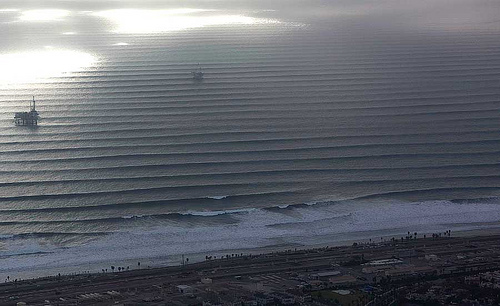
\includegraphics{bilder/swell}
    \caption{Linienförmig eintreffender Swell}
  \end{center}
\end{figure}

Wellen entstehen dadurch, dass die Wasseroberfläche durch die über ihr
strömenden Winde in Bewegung versetzt wird. Die Gipfel und Täler der
Wellen werden durch die Zirkulation des Windes über der Oberfläche
immer höher und tiefer, bis sie ein Limit erreichen und wieder in sich
zusammenbrechen. Die Höhe der Wellen ist dabei von der Stärke, der
Dauer und der Lauflänge \footnote{die Strecke über der Wind strömt}
des Windes abhängig.

Die so erzeugten Wellen breiten sich dann vom Entstehungsort
kreisförmig auf ihre Umgebung im Meer aus. Die Geschwindigkeit ist
dabei abhängig von der \textit{Wellenlänge}, dem Abstand zwischen zwei
Wellengipfeln. Das Wellenchaos am Entstehungsort mit vielen
unterschiedlichen Wellenlängen beginnt sich mit der Ausbreitung zu
legen. Die schnelleren Wellen, mit weiter auseinander liegenden
Gipfeln, beginnen die langsameren Wellen zu überholen und fangen an
sich linienförmig zu ordnen. Die vorderen Wellen werden dabei zu den
kräftiger und sauber angeordneten, die hinteren Wellen zu den
schwächeren und chaotischeren. Je weiter die Strecke die ein Swell
hinter sich gelegt hat und linienförmiger er geordnet ist, desto
größer ist die Geschwindigkeit und die Kraft der Wellen am Ort an dem
sie brechen.

Swell ist eine der Grundvoraussetzungen für gute und surfbare
Wellen. Deshalb gibt es z.B. auch in Deutschland keine guten
Surfspots, da der potentiell eintreffende Swell meistens durch England
abgeschirmt wird.

\section{Voraussetzungen zum Surfen}

\section{Ziel der Diplomarbeit}

Ziel der Diplomarbeit ist die Entwicklung einer \textit{Community
  Plattform} für Surfer, welche den Grundgedanken der
\textit{Stormrider Guides} aufgreift, mit den neuen Möglichkeiten des
Internets und des Web 2.0 verknüpft, und somit einen Mehrwert für
Surfer generiert. Grundlage der Plattform sollen Beschreibungen und
Kommentare der Mitglieder zu den verschiedenen Surf Spots sein. Diese
werden dann mit anderen Diensten wie \textit{Google Maps},
\textit{Flickr} und \textit{YouTube} verknüpft. Außerdem sollen
Wetter- und Wellenvorhersagen für die verschiedenen Spots integriert
werden, um aktuelle Informationen zu den Surfbedingungen
bereitzustellen.

Die bei der Konzeption und Implementierung aufgetretenen Probleme und
Lösungen werden in dieser Arbeit vorgestellt.



% 
{\sf \footnotesize
  \begin{tabular}{|p{2.5cm}p{0.7cm}p{0.7cm}|}
    \hline
    & & \\
    \multicolumn{3}{|l|}{\textbf{Hai Angriff Statistik}} \\
    \multicolumn{3}{|l|}{für Länder mit mehr als 10 Angriffen} \\
    & & \\
    & \textbf{Tota}l & \textbf{Fatal} \\
    \textbf{Europa} & \textbf{38} & \textbf{18} \\
    Italien & 14 & 4 \\
    \textbf{Afrika} & \textbf{255} & \textbf{67} \\
    Südafrika & 208 & 41 \\
    Mosambik & 11 & 3 \\
    \textbf{Indischer Ozean} & \textbf{62} & \textbf{27} \\
    Maskarenen & 21 & 12 \\
    Iran & 23 & 8 \\
    Indien & 10 & 4 \\
    \textbf{Ost Asien} & \textbf{89} & \textbf{38} \\
    Papua-Neuguinea & 36 & 15 \\
    Philippinen & 15 & 6 \\
    Japan & 19 & 12 \\
    \textbf{Australien \& Neuseeland} & \textbf{326} & \textbf{141} \\
    West Australien & 28 & 9 \\
    Süd Australien & 30 & 16 \\
    Victoria & 20 & 8 \\
    Tasmanien & 16 & 6 \\
    Neusüdwales & 123 & 62 \\
    Queensland & 101 & 47 \\
    \textbf{Pazifik} & \textbf{211} & \textbf{62} \\
    Marshallinseln & 12 & 0 \\
    Salomon-Inseln & 17 & 8 \\
    Fiji & 25 & 10 \\
    Hawaii & 104 & 19 \\
    \textbf{Nord Amerika} & \textbf{720} & \textbf{38} \\
    Oregon & 17 & 1 \\
    Kalifornien & 111 & 8 \\
    Texas & 30 & 3 \\
    Florida & 187 & 13 \\
    Südkarolina & 43 & 3 \\
    Nordkarolina & 24 & 3 \\
    New Jersey & 16 & 5 \\
    \textbf{Zentralamerika} & \textbf{118} & \textbf{50} \\
    Mexiko & 39 & 21 \\
    Panama & 16 & 9 \\
    \textbf{Südamerika} & \textbf{89} & \textbf{21} \\
    Brasilien & 81 & 20 \\
    & & \\
    \textbf{TOTAL} & \textbf{1909} & \textbf{456} \\
    & & \\
    \multicolumn{3}{|l|}{The International Shark Attack File,} \\
    \multicolumn{3}{|l|}{Florida Museum of Natural History,} \\
    \multicolumn{3}{|l|}{University of Florida.} \\
%    \multicolumn{3}{|l|}{{\tiny http://www.flmnh.ufl.edu/fish/Sharks/ISAF/ISAF.htm}} \\
    \hline
  \end{tabular}
}

%%% Local Variables:
%%% mode: latex
%%% TeX-master: "../community-plattform"
%%% End:


%%% Local Variables:
%%% mode: latex
%%% TeX-master: "../community-plattform"
%%% End:

%
\chapter{Anforderungen an die Web Applikation}

\section{Spot Beschreibungen}

Eine der bekanntesten Wellen in Europa ist im spanischen Baskenland an
einer Fluss\-mündung östlich des Ortes \textit{Mundaka} zu finden. Im
\textit{Stormrider Guide Europe} \cite[S.180]{storm_europe_1998}
werden die Surfbedingungen an diesem Spot wie folgt beschrieben.

\textit{Some of the longest, hollowest lefts in Europe break over
  sandbanks at the mouth of the river Gernike. It's best at low tide,
  when the rivers current (a useful conveyor belt) is less intense,
  and holds swell up to 4m (12ft). On the other side of the rivermouth
  are the beaches Laida and Laga where you can find waves at small
  swells. The river and its estuary are a Worldwide Fund for Nature
  reserve, but even so, the water is not as clean as could expected.
}

Zusätzlich werden den Beschreibungen Piktogramme aus verschiedenen
Kategorien zugeordnet, welche die Gegebenheiten vor Ort durch eine
vereinfachte grafische Darstellung widerspiegeln. Einige dieser
Kategorien sind die bevorzugte Windrichtung, die optimale Gezeit, die
Art der brechenden Welle, Beschaffenheit des Bodens, sowie mögliche
Gefahren. Kennt man einmal die Piktogramme, ist durch einen kurzen
Blick schnell ersichtlich welche Bedingungen an einem Spot herrschen.

\begin{figure}[h]
  \begin{center}
    
\includegraphics[height=40px]{bilder/mundaka-conditions}
    \caption{Piktogramme zu den Surfbedingungen in Mundaka}
    \label{piktogramm}
  \end{center}
\end{figure}


In Abbildung \ref{piktogramm} sind die Piktogramme zu sehen, die für
die obige Beschreibung in Mundaka verwendet wurden. Sie sollen
vermitteln, dass dieser Spot sehr bekannt ist und an guten Tagen mit
vielen Surfern zu rechnen ist. Die Welle bricht mit viel Kraft von
links nach rechts (\textit{Left-hander}, immer vom Strand aus gesehen)
über einer Sandbank, wobei vereinzelt Surfbretter zu Bruch gehen
können.  Sie ist nicht bei Flut (\textit{High Tide}) surfbar, und
ablandiger Wind (\textit{Offshore}) aus dem Süden trägt dazu bei, dass
die Wellen geglättet werden, später brechen und hohler werden.

Das Konzept der Stormrider Guides soll die Grundlage der Web
Applikation bilden und mit den neuen Möglichkeiten des Internets
verknüpft werden. Die Beschreibungen zu den Spots und deren
Gegebenheiten sollen gemeinschaflich durch die Mitglieder der Surf
Community verfasst werden, und als sogenannter \textit{User Generated
  Content} verwaltet werden. Die gemeinsam erstellten Beschreibungen
sollen eine objektive Sicht auf die Gegebenheiten und Surfbedingungen
an den jeweiligen Spots bieten. Für persönliche Ansichten und
Diskussionen sollen Kommentarfunktionen zur Verfügung gestellt werden
die in Abschnitt \ref{subsec:Kommentare} beschrieben werden.

Um Spam und anderer mutwilliger Zerstörung oder Verunreinigung des
Contents vorzubeugen ist eine Registrierung der Nutzer
erforderlich. Für alle Informationen die zu einem Spot gehören und von
Nutzern der Web Applikation verändert werden können, soll eine
Historie verwaltet werden. Dies soll sicherstellen, dass bei einer
eventuellen Veruneinigung des Contents auf eine frührere Version der
Information zurückgegriffen, und diese wiederhergestellt werden kann.

\section{Kartenmaterial}

Um das Auffinden von Spots zu vereinfachen sollen diese auf einer
Karte dargestellt werden. Webservice Dienste wie \textit{Google Maps},
\textit{Yahoo! Maps} oder Microsoft's \textit{Bing Maps}
\footnote{seit Juni 2009, früher: Microsoft's Virtual Earth} bieten
die Möglichkeit interaktive Karten per Java\-script oder Flash in eine
Webseite einzubetten. Diese Dienste bieten nicht nur die typischen
Land- bzw. Straßenkarten an, sondern stellen auch Satelitenbilder und
teilweise 3-dimensionale Ansichten für bestimmte Gebiete zur
Verfügung.

\section{Wetter- und Wellendaten}
\label{sec:Wetter- und Wellendaten}

Wie schon in der Einleitung erwähnt ist das Vorhandensein von Swell
eine der Grundvoraussetzungen zum Surfen. Viele Surfer nutzen deshalb
regelmäßig Dienste im Internet um sich über die Wetter- und
Wellenverhältnisse in den nächsten Tagen zu informieren. Dabei ist
hauptsächlich die Wellenhöhe, die Wellenperiode und die Stärke und
Richtung des Windes von Interesse. Die Spot Beschreibungen sollen
deshalb mit aktuellen Wetter- und Wellenvorhersagen verknüpft werden,
um den Benutzern der Web Applikation einen Mehrwert zu bieten. Die
\textit{National Oceanic and Atmospheric Administration (NOAA)} ist
die Wetter- und Ozeanografiebehörde der Vereinigten Staaten. Sie
besteht aus 5 größeren Organisationen, zu denen unter anderen auch der
\textit{National Weather Service} und der \textit{National Ocean
  Service} gehören, welche die benötigten Wetter- und Wellendaten zur
Verfügung stellen. Viele der im Internet verfügbaren Dienste, die
Wetter- oder Wellenvorhersagen anbieten, beziehen ihre Daten ebenfalls
von diesen Organisationen.

\section{Bilder \& Videos}

Um Surfern einen visuellen Eindruck von einem Spot zu bieten, sollen
die Spots mit Bildern und Videos verknüpft und somit aufgewertet
werden. Auf Internetseiten wie \textit{Flickr} und \textit{YouTube}
sind von vielen bekannten Spots Bilder und Videos zu finden. Eine
Suchanfrage nach einem der bekanntesten Spots mit den Stichwörtern
\textit{Mavericks} und \textit{Surf} ergab im Juni 2009 bei
\textit{Flickr} 2319 und bei \textit{YouTube} 548 Ergebnisse. Diese in
der Surf Community gerne gesehenen Bilder und Videos sind ideal um das
bisher aus Beschreibungen und Wetter-/Wellenvorhersagen bestehende
Informationsangebot zu erweitern. Sowohl \textit{Flickr} als auch
\textit{YouTube} bieten eine Webservice Schnittstelle an, mit der es
möglich ist deren Bilder und Videos in eigene Anwendungen zu
integrieren. Zudem soll den Nutzern die Möglichkeit gegeben werden
ihre eigenen Bilder und Videos auf die Community Plattform zu laden
und dort zu veröffentlichen.

\section{Community Funktionen}

Einige Funktionen, die aus Community Plattformen wie \textit{Facebook}
und \textit{StudiVZ} bekannt sind sollen auch in dieser Web
Applikation zu Verfügung stehen. Ziel ist auch hier einen Mehrwert für
die Nutzer zu generieren, um diese näher an die Plattform zu binden.

\subsection{Freundschaften}
Nutzer sollen in der Lage sein Freundschaftsanfragen an andere Nutzer
zu stellen, und Anfragen anderer Nutzern zu akzeptieren
bzw. abzulehnen.

\subsection{Nachrichten}

\subsection{Kommentare}
\label{subsec:Kommentare}

Spot Beschreibungen sollen eine objektive Sicht auf die


\subsection{Secret Spots}

%%% Local Variables:
%%% mode: latex
%%% TeX-master: "../community-plattform"
%%% End:


\chapter{Einleitung}
\section{Motivation}
\section{Die Entstehung von Wellen}
\section{Voraussetungen zum Surfen}
\section{Ziel der Diplomarbeit}

\chapter{Anforderungen an die Web Applikation}
\section{Wetter- und Wellendaten}
\section{Kartenmaterial}
\section{Community Funktionen}

\chapter{Implementierung der Web Applikation}
\section{Vorstellung der verwendeten Technologien}
\section{Behavior Driven Development}
\section{Architektur der Web Applikation}
\section{Caching Verfahren in Ruby on Rails}

\chapter{Aufbau und Analyse der ETL Prozesse}
\section{Überblick der verwendeten Datenquellen}
\subsection{Wetterdaten}
\subsection{Photos \& Videos}
\section{Datenbank Design}
\subsection{Konzeptionelle Schema}
\subsection{Physisches Schema}
\section{Extraktion aus den Quellsystemen}
\section{Transformation der Daten}
\section{Laden der Daten}
\section{Verbesserungen}

\chapter{Ausblick}
\section{Visualisierung von Wetter- und Wellendaten}
\section{Data Mining Verfahren}

\bibliographystyle{geralpha}
\bibliography{literatur}

\end{document}